\chapter{Background}
\label{chap:background}

% Describe what we need to understand to move forward
In order to properly discuss the BB84 quantum KEP one must first understand some basic principals and terminology of encryption, quantum computation, and how they affect one another. 
This foundation will allow us to critically analyze and understand the properties and intricacies of the protocol.

\section{Encryption}
\subsection{Symmetric Encryption}
% Symmetric Encryption
Symmetric encryption is what comes to most people's mind when they think of encryption.
It is encryption in which both the encrypter and decrypter, Alice and Bob, use the same key (a number or series of bits used for a cryptographic algorithm).
While symmetric encryption is the oldest form of encryption, being used for over 4000 years, it does have a major drawback, the key distribution problem: if Alice and Bob are separate parties (as in the case of secure message transmission), they must exchange their key beforehand using a secure channel \cite{cryptography}.
If an eavesdropper, Eve, were to intercept the key in transit then the encryption is compromised and there is not necessarily any way for Alice or Bob to know.

% One Time Pad in depth
A One-Time-Pad (OTP) is a symmetric key that is only used once.
The OTP is shared between both Alice and Bob, used to encrypt and decrypt a single message, and then discarded.
The OTP is usually the same length as the message it encrypts, so bit-wise encryption techniques, such as parity manipulation, can add the the security of the key.
Under the proper conditions, a OTP is considered to be ``perfect encryption", and it is only susceptible to brute forcing, which is of course usually infeasible given a sufficiently large key \cite{cryptography}.
% One Time Pad caveats
OTPs suffer from the same issue as all symmetric encryption protocols, the key distribution problem, making it highly impractical in many cases.

\subsection{Asymmetric Encryption}
% Asymmetric encryption
Asymmetric encryption, also known as public-key cryptography, solves this problem as far as classical computers are concerned.
It is is the process of encrypting data using one key in such a way that it can be decrypted using a different key.
In effect, Alice, can encrypt a message using a key that is publicly accessible, and the message can only be decrypted by Bob, who has the secret key corresponding to the public key used.
This method requires a key to be compromised of two parts, a public and private key-pair: $k = (k_{pub}, k_{priv})$ where $k_{pub} = f(k_{priv})$ \cite{cryptography}.


% Diffie Hellman in depth
The Diffie-Hellman KEP was the first asymmetric KEP to be proposed, and is still widely used in various forms today. 
It is performed as follows:

\begin{enumerate}
\item Some large prime $p$ and an integer $\alpha \in \{2,3,4,...,p-2\}$ are shared.
\item Each party, Alice and Bob, computes their own keys: $k_{priv,X} = x \in \{2,3,4,...,p-2\}$ and $k_{pub, X} = X =  \alpha^x mod p$.
\item Alice and Bob exchange their public keys, $X \in \{A, B\}$, respectively. 
\item Alice and Bob each compute a session key $k_{AB} = A^b mod p$ or $k_{AB} = B^a mod p$. Because $(\alpha^a)^b = (\alpha^b)^a = \alpha^{ab}$, both Alice and Bob end with the same session key despite never knowing each other's private keys. 
\end{enumerate}

This method is cryptographically secure due to the Discreet Logarithm Problem (DLP), finding $x$ such that $B = \alpha^x$. 
This problem is computationally not feasible to solve using classical computers, making the Diffie-Hellman KEP and other KEP based off of the DLP or prime factorization secure against any attacks by a classical computer \cite{qc:agi}.

\section{Quantum Computation}

% Basic properties
Just as classical computation involves bits, quantum computation is computation using quantum bits, qubits, denoted $\ket{\psi}$. 
%	State
It is commonly said that while a classical bit exists in either the state 1 or 0, qubits can exist in both  $\ket{0}$ and $\ket{1}$ at once.
There is an element of truth in this, but a more accurate description would be that a qubit has a state vector that exists in a 3-dimensional complex state-space. 
There is a lot to unpack here, but it becomes a bit more clear when we examine the state space in 2 dimensions.
\begin{figure}[htp]
\centering
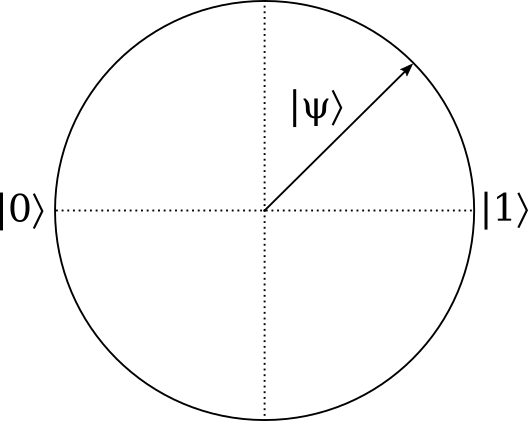
\includegraphics[scale=.25]{images/standard_basis.png}
\caption{State vector in a 2-D state space}
\label{Standard basis circle}
\end{figure}
The state of a qubit rather exists somewhere in between $\ket{0}$ and $\ket{1}$ \cite{qc:agi}.
%	Measurement
Just as a computer can read the value of a classical bit, when we measure the qubit against $\ket{0}$ and $\ket{1}$ its state collapses to one of the two.
The probability with which a vector will collapse into one of two states is defined as $\ket{\psi} = \alpha\ket{0} + \beta\ket{1}$, where $|\alpha|^2 + |\beta|^2 = 1$.
We use quantum gates or operators to manipulate $\alpha$ and $\beta$ probabilities.
For example, the Hadamard Gate, or H gate, performs what is called a "quarter turn"; it maps $\ket{\psi} = \ket{0} \Rightarrow \ket{\psi} = \frac{1}{\sqrt{2}}\ket{0} + \frac{1}{\sqrt{2}}\ket{1}$ and $\ket{\psi} = \ket{1} \Rightarrow \ket{\psi} = \frac{1}{\sqrt{2}}\ket{0} - \frac{1}{\sqrt{2}}\ket{1}$ \cite{qc:agi}.
Since after the H gate is applied $\alpha$ and $\beta$ both equal $\frac{1}{\sqrt{2}}$, and ${\frac{1}{\sqrt{2}}}^2 = \frac{1}{2}$, if we measure $\ket{\psi}$ in this state it would collapse to $\ket{0}$ and $\ket{1}$ with equal probability. 
It is worth noting this is one way to create a true-random number generator.

%	Bases
Because the state vector exists in a 3D state space, we do not necessarily have to measure against $\ket{0}$ and $\ket{1}$, in fact we can measure against any two vector values that are opposite each other on the unit circle. 
A set of vectors to measure against is known as a basis, and there are many possible bases. 
The set $\{\ket{0},\ket{1}\}$ is known as the standard basis or computational basis, as it is analogous to classical bits \cite{qcftgu}.
Another common basis is the Hadamard Basis, which is denoted $\ket{+} = \frac{1}{\sqrt{2}}\ket{0} + \frac{1}{\sqrt{2}}\ket{1}$ and $\ket{-} = \frac{1}{\sqrt{2}}\ket{0} - \frac{1}{\sqrt{2}}\ket{1}$.
The H gate will put $\ket{0} \Rightarrow \ket{+}$ and $\ket{1} \Rightarrow \ket{-}$, but it will also revert the Hadamard basis into the standard basis: $\ket{+} \Rightarrow \ket{0}$ and $\ket{-} \Rightarrow \ket{1}$.
Because the standard basis and the Hadamard basis are perpendicular to each other they are referred to as orthonormal bases.
That is to say if a $\ket{\psi} = \ket{+}$ or $\ket{\psi} = \ket{-}$ then it will have 50\% of being $\ket{0}$ or $\ket{1}$ if measured in the standard basis, and vice-versa. 

\begin{figure}[htp]
\centering
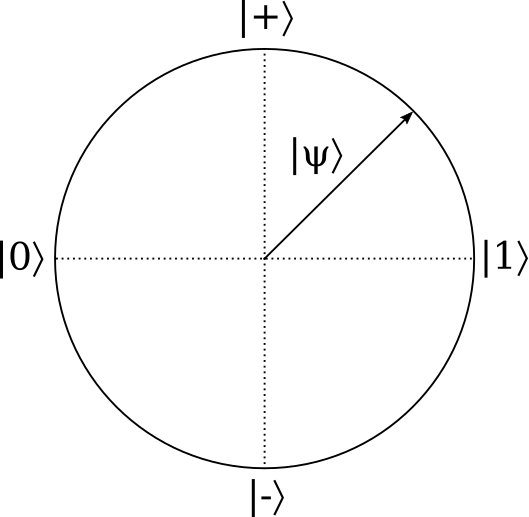
\includegraphics[scale=0.25]{images/orthonormal_basis.png}
\caption{A state vector with the Hadamard and standard bases in as 2D state space}
\label{}
\end{figure}

In effect if you have a vector in one orthonormal basis it is useless if measured in another orthonormal basis.
Further, since the vector state changes when measured, if a value is encoded in one orthonormal basis, that information is destroyed by measuring in another orthonormal basis. 

% Guarantees
% 	Copy-ability
Another crucial property of qubits is that they cannot be cloned.
It is impossible to have an operator that clones the state of an input qubit into an output qubit.
This property proves crucial in the BB84 protocol, as explained in Chapter~\ref{chap:bb84}.

Using these properties and others, it has been shown that quantum computers can factor large prime numbers in order $\sqrt{N}$ time.
With this in mind, and the growing power of quantum computers, the securities of the Diffie-Hellman and asymmetric encryption are threatened.
The BB84 protocol is a quantum key distribution (QKD) protocol that allows two parties to co-create a shared key, using a verifiably secure channel, that can then be used to symmetrically encrypt messages.